\input preamble.tex
\noindent
\section*{Laboppgave Mal}

\vskip 5pt
%beskrivelse av oppgaven
I denne laboppgaven skal du....

Før du  starter må du......
\begin{itemize}[noitemsep]
	\item --
\end{itemize}

\vskip 5pt 
Valgfrie oppdrag:

\vskip 5pt 
\begin{itemize}[noitemsep]
	\item --
\end{itemize}



\vskip 2.5pt 
%kompetansemål som oppgaven dekker
Kompetansemål:
\begin{itemize}[noitemsep]

	\item utføre risikovurdering og vurdere tiltak som skal ivareta person- og maskinsikkerheten, i henhold til hvilke regelverk og normer som gjelder for arbeidet som skal utføres
	\item utføre arbeid på automatiserte anlegg fagmessig, nøyaktig og i overensstemmelse med gjeldende regelverk og normer for elektriske installasjoner og maskiner
	\item planlegge, gjennomføre, vurdere kvalitet, sluttkontrollere og digitalt dokumentere arbeidsoppdragene i faget automatiseringssystemer, individuelt og i samarbeid med andre, og begrunne valgene som er gjort
	\item tegne tekniske flytskjemaer og annen dokumentasjon, og anvende dette i utførelsen av alle arbeidsoppdrag
	\item utføre vedlikehold, systematisk feilsøking og feilretting med egnede instrumenter og verktøy, og vurdere måleresultater opp mot forventede og beregnede verdier
	\item montere, konfigurere, kalibrere, justere og sette i drift reguleringssløyfer for motor- og servodrift, temperatur, trykk, nivå og strømning, og simulere og optimalisere regulatorer basert på prosessbehov og gjøre rede for funksjon og virkemåte
	\item gjøre rede for måleprinsipper for veiing, deteksjon med kamera, vibrasjon, gassdekteksjon, pH-måling og konduktivitet for analyse og montere, konfigurere, kalibrere, justere og sette i drift minst ett av disse målesystemene
	\item montere og sette i drift ulike typer pådragsorganer med tilhørende forstillingselementer og hjelpeutstyr i henhold til leverandørens dokumentasjon, og gjøre rede for hvordan utstyret fungerer, og hvilke funksjoner det har
	\item montere og sette i drift sikkerhetskomponenter og -utstyr for nødstopp- og sikkerhetskretser, og gjøre rede for sikkerhetskategoriene Safety Integrity Level (SIL) og Performance Level (PL)
	\item programmere, montere og sette i drift programmerbare styresystemer for elektriske-, pneumatiske- og hydrauliske anlegg og gjøre rede for hvordan utstyret fungerer, og hvilke funksjoner det har
	\item installere bus-systemer og konfigurere digital og analog kommunikasjon i automatiserte anlegg, og gjøre rede for hvordan komponentene fungerer, hvordan datasignaler bearbeides og transporteres mellom nettverk, og vurdere tiltak for å etablere et sikkert elektronisk kommunikasjonsnett
	\item installere, terminere og skjøte elektriske og optiske kabler og måle kvaliteten på forbindelsen og beskrive faktorer som påvirker kvaliteten på forbindelsen
	\item installere, programmere, konfigurere og brukertilpasse «Human–Machine Interface» (HMI) for et automatiseringssystem og gjøre rede for bruksområdene
	\item simulere, sette i drift, programmere og optimalisere robot og gjøre rede for roboters funksjon og anvendelse i automatiserte anlegg
	\item foreslå, vurdere og utprøve forenklinger og forbedringer av produkter og produksjonsprosesser og gjøre rede for mulig bruk i nye produkter og tjenester
	\item håndtere avfall etter eget arbeid i industrielle og automatiserte anlegg på en miljøvennlig og økonomisk måte, drøfte produkters miljøprestasjon, slette sensitiv informasjon ved avhending og gjøre etiske og økonomiske refleksjoner rundt bærekraft, sirkulær økonomi og produktkvalitet
	\item diskutere verdien av å oppleve mestring og stolthet over eget arbeid og av å oppleve tilhørighet og trygghet i et arbeidsmiljø uavhengig av kjønn og kultur
	\item reflektere over bedriftsdemokratiets og det organiserte arbeidslivets forutsetninger, verdier og regler og hvordan et regulert arbeidsliv kan bidra til å motvirke arbeidslivskriminalitet, diskriminering og forskjellbehandling
	\item dokumentere eget arbeid, vurdere arbeidsmetoder, faglige løsninger, kvalitet og estetikk i arbeidsoppdraget, foreslå forbedringer og reflektere rundt mulige endringer




\end{itemize}

%anbefalt lesning til arbeidsoppdragene
Anbefalt lesning:

\begin{enumerate}
	\item afgv.pdf/ 
\end{enumerate}

%Liste over oppdrag som skal gjøres med ruter for godkjennening

%\begin{center}
%\begin{tabular}{ | m{10cm} | m{1cm}| m{2cm} | } 
%\hline
%\multicolumn{3}{|c|}{Liste over oppgaver som skal utføres} \\
%	\hline
%	Oppgave	& Utført & Signatur \\ 
%	\hline
%	\hline
%	(Nivå 1)	& & \\ 
%	\hline
%	(Nivå 2)	& & \\ 
%	\hline
%	(Nivå 3)	& & \\ 
%	\hline
%	(Nivå 4)	& & \\ 
%	\hline
%\end{tabular}
%\end{center}

%--------------------------------------
\newpage

\subsection*{Oppgave 1 -  Oppkobling av HC-SR04}
I denne oppgaven skal vi bli kjent med ultralydsensoren HC-SR04. Denne sensoren sender ut en ultralyd puls når Trig pinnen akriveres (10µs puls), sammtidig som trig pinnen aktiveres slås echo pinnen på, den står på til vi mottar et retur signal (reflektert lyd)

$$\includegraphics[width=9cm]{lUltralydtransmitterx03.eps}$$
I vårt program kan vi bruke funksjonen \verb|pulseIn()|. Denne funksjonen tar tiden på hvor lenge en variabel (echo pinnen) har vært høy. Den virker på pulser fra 10µs til 3 minutter. Tiden den returnerer er i µs. 
\vskip 2.5pt 

\underbar{file ./lUltralydtransmitter.tex}
\vskip 5pt 

\end{document}

